\documentclass[tikz,border=10pt]{standalone}
\usepackage{amsmath}
\usetikzlibrary{calc,angles,quotes}
\begin{document}
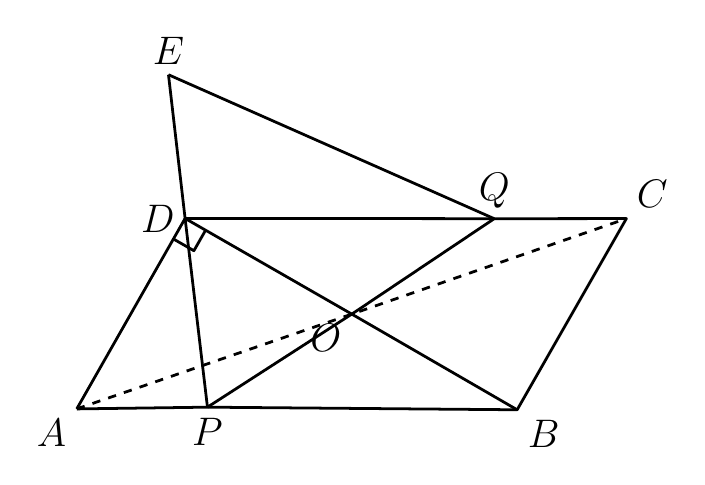
\begin{tikzpicture}[line join=round, line width=1.0pt,
  lbl/.style={font=\fontsize{13.5}{16.2}\selectfont}]
\coordinate (A) at (-3.496,-2.101);
\coordinate (B) at (2.097,-2.112);
\coordinate (C) at (3.484,0.316);
\coordinate (D) at (-2.120,0.318);
\coordinate (E) at (-2.331,2.143);
\coordinate (O) at (-0.003,-0.897);
\coordinate (P) at (-1.836,-2.079);
\coordinate (Q) at (1.806,0.315);




\draw (A)--(P)--(B)--(C)--(Q)--(D)--(A);

\draw (D)--(O)--(B);

\draw (P)--(O)--(Q);

\draw (E)--(Q);
\draw (E)--(D)--(P);

\draw[dashed] (A)--(O)--(C);


\draw pic[draw,angle radius=0.300cm] {right angle=A--D--O};


\node[lbl,above] at (E) {$E$};
\node[lbl,left] at (D) {$D$};
\node[lbl,above] at (Q) {$Q$};
\node[lbl,above right] at (C) {$C$};
\node[lbl,below left] at (A) {$A$};
\node[lbl,below] at (P) {$P$};
\node[lbl,below right] at (B) {$B$};
\node[lbl,below left] at (O) {$O$};
\end{tikzpicture}
\end{document}